% CampusWatch campus in Cisco Packet Tracer. Build:  tectonic docs/Packet_Tracer_Topology.tex
\documentclass[11pt,a4paper]{article}

\usepackage{fontspec}
\setmainfont{texgyrepagella}[Extension=.otf, UprightFont=*-regular, BoldFont=*-bold, ItalicFont=*-italic, BoldItalicFont=*-bolditalic]
\setsansfont{texgyreheros}[Extension=.otf, UprightFont=*-regular, BoldFont=*-bold, ItalicFont=*-italic, BoldItalicFont=*-bolditalic]
\setmonofont{lmmono10-regular.otf}

\usepackage[margin=2.2cm, headheight=14pt]{geometry}
\usepackage{xcolor}
\usepackage{tikz}
\usetikzlibrary{positioning, arrows.meta, fit, backgrounds, calc}
\usepackage[most]{tcolorbox}
\usepackage{booktabs, tabularx, array}
\usepackage{listings}
\usepackage{enumitem}
\usepackage{titlesec}
\usepackage{fancyhdr}
\usepackage{amsmath, amssymb}
\usepackage{needspace}
\usepackage[hidelinks]{hyperref}

\definecolor{ink}{HTML}{1B2430}
\definecolor{muted}{HTML}{5B6676}
\definecolor{accent}{HTML}{1F9FBC}
\definecolor{rule}{HTML}{D5DBE3}
\definecolor{codebg}{HTML}{F4F6F9}
\definecolor{acad}{HTML}{3987E5}
\definecolor{admin}{HTML}{D95926}
\definecolor{stu}{HTML}{199E70}
\definecolor{dc}{HTML}{9085E9}
\definecolor{warnc}{HTML}{C98500}
\definecolor{okc}{HTML}{1E9E5A}

\hypersetup{colorlinks=true, linkcolor=accent, urlcolor=accent}
\setlength{\parindent}{0pt}
\setlength{\parskip}{6pt}
\setlength{\emergencystretch}{3em}
\renewcommand{\arraystretch}{1.25}
\setlist{itemsep=2pt, topsep=4pt}

\titleformat{\section}{\sffamily\Large\bfseries\color{ink}}{\thesection}{0.8em}{}[\vspace{-2pt}{\color{rule}\titlerule}]
\titleformat{\subsection}{\sffamily\large\bfseries\color{ink}}{\thesubsection}{0.7em}{}
\titlespacing*{\section}{0pt}{16pt}{8pt}

\pagestyle{fancy}
\fancyhf{}
\fancyhead[L]{\sffamily\small\color{muted}CampusWatch campus in Cisco Packet Tracer}
\fancyhead[R]{\sffamily\small\color{muted}Build guide}
\fancyfoot[C]{\sffamily\small\color{muted}\thepage}
\renewcommand{\headrulewidth}{0.4pt}
\renewcommand{\headrule}{\color{rule}\hrule width\headwidth height\headrulewidth}

\lstdefinestyle{ios}{basicstyle=\ttfamily\small, backgroundcolor=\color{codebg}, frame=single, rulecolor=\color{rule},
  framesep=6pt, xleftmargin=6pt, xrightmargin=6pt, columns=fullflexible, keepspaces=true, breaklines=true,
  showstringspaces=false, aboveskip=6pt, belowskip=8pt, commentstyle=\color{muted}, morecomment=[l]{!}}
\lstset{style=ios}

\newtcolorbox{note}[1][Note]{colback=warnc!7, colframe=warnc, boxrule=0.6pt, arc=2pt, left=8pt, right=8pt, top=4pt,
  bottom=4pt, fonttitle=\sffamily\bfseries\small, coltitle=white, title=#1}
\newtcolorbox{tip}[1][Tip]{colback=okc!6, colframe=okc, boxrule=0.6pt, arc=2pt, left=8pt, right=8pt, top=4pt,
  bottom=4pt, fonttitle=\sffamily\bfseries\small, coltitle=white, title=#1}
\newcommand{\code}[1]{\texttt{#1}}

\newcolumntype{Y}{>{\raggedright\arraybackslash}X}
\let\oldsection\section\renewcommand{\section}{\needspace{12\baselineskip}\oldsection}
\let\oldsubsection\subsection\renewcommand{\subsection}{\needspace{8\baselineskip}\oldsubsection}
\begin{document}

\begin{center}
{\sffamily\color{accent}\large CampusWatch\par}
\vspace{2pt}
{\sffamily\bfseries\LARGE\color{ink} The campus topology in Cisco Packet Tracer\par}
\vspace{6pt}
{\color{muted} Devices, cabling, IOS configurations and verification for Packet Tracer 8.x\par}
\end{center}

This guide builds the CampusWatch campus in Packet Tracer. It uses the dashboard's demo device names, VLANs and IP addresses,
so you can show the same network in both. Allow 30 to 40 minutes. Paste each configuration block into the device's
\textbf{CLI} tab (or \textbf{Config $\rightarrow$ CLI}).

\begin{note}[Why the dashboard does not poll Packet Tracer]
Packet Tracer is a simulation: its devices exist only inside the program, so CampusWatch running on your laptop cannot reach
them. Demonstrate SNMP from inside Packet Tracer with a PC's \textbf{MIB Browser} (Section 6), then show the dashboard in Demo
mode, which uses the same campus and labels its data as synthetic.
\end{note}

% ------------------------------------------------------------------
\section{Topology}

\begin{center}
\resizebox{\linewidth}{!}{%
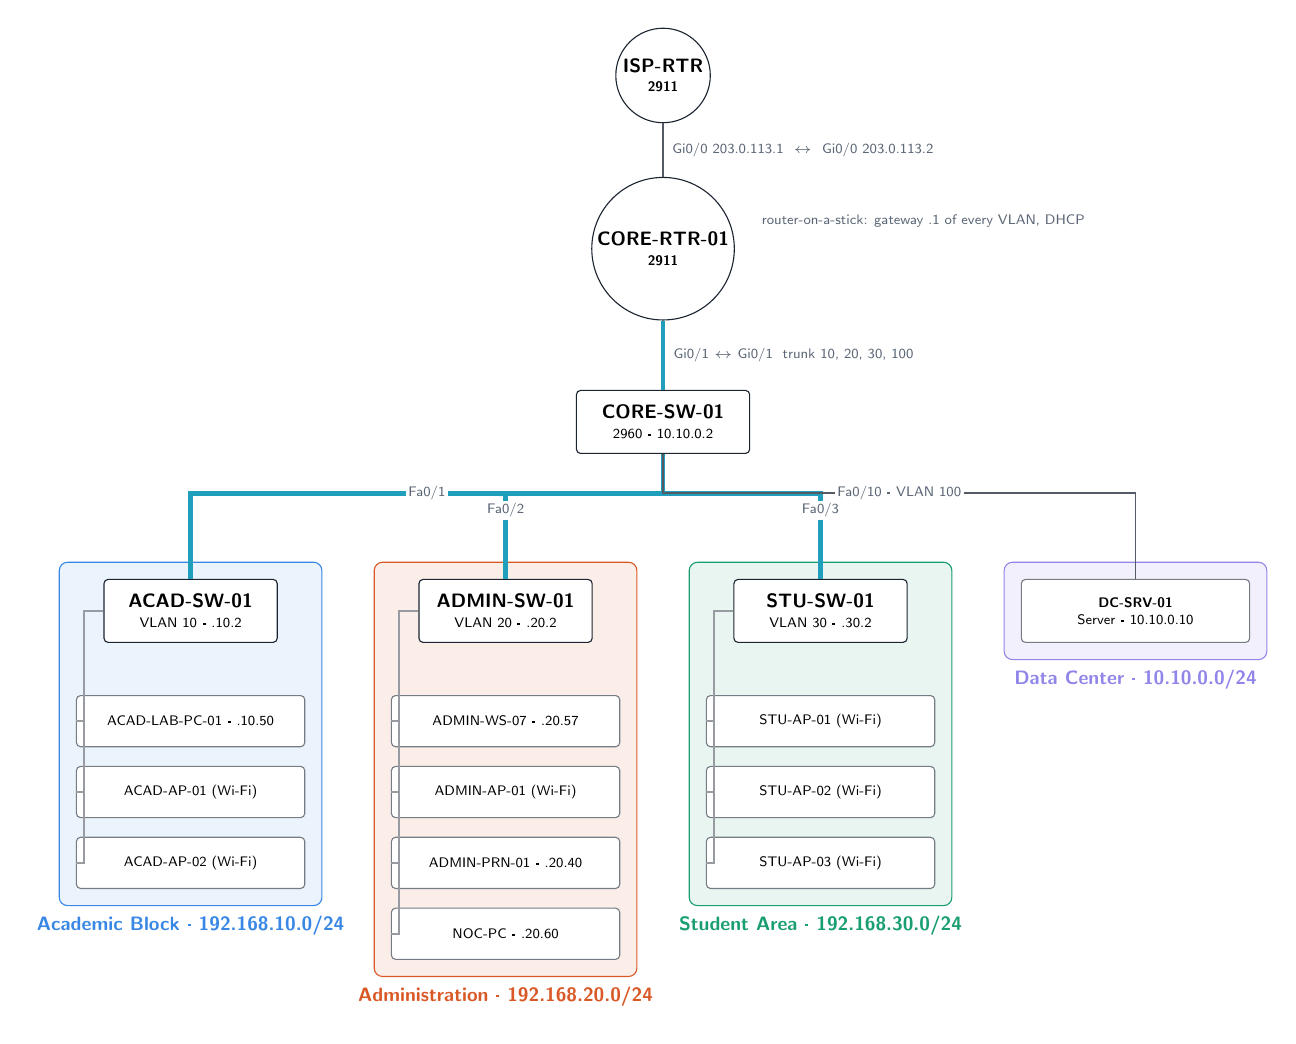
\begin{tikzpicture}[
  font=\sffamily\scriptsize,
  rtr/.style={draw=ink, fill=white, circle, minimum size=12mm, inner sep=1pt, align=center, font=\sffamily\scriptsize\bfseries},
  sw/.style={draw=ink, fill=white, rectangle, rounded corners=1.5pt, minimum width=22mm, minimum height=8mm, align=center, font=\sffamily\scriptsize\bfseries},
  host/.style={draw=ink!60, fill=white, rectangle, rounded corners=1.5pt, minimum width=29mm, minimum height=6.5mm, align=center, font=\sffamily\tiny},
  link/.style={draw=ink!75, line width=0.7pt},
  trunk/.style={draw=accent, line width=1.6pt},
  lbl/.style={font=\sffamily\tiny, text=muted, fill=white, inner sep=1pt}]

  \node[rtr] (isp) at (0,0) {ISP-RTR\\[-1pt]\tiny 2911};
  \node[rtr] (core) at (0,-2.2) {CORE-RTR-01\\[-1pt]\tiny 2911};
  \node[sw] (csw) at (0,-4.4) {CORE-SW-01\\[-1pt]\tiny\mdseries 2960 · 10.10.0.2};

  \node[sw] (acad) at (-6,-6.8) {ACAD-SW-01\\[-1pt]\tiny\mdseries VLAN 10 · .10.2};
  \node[sw] (adm)  at (-2,-6.8) {ADMIN-SW-01\\[-1pt]\tiny\mdseries VLAN 20 · .20.2};
  \node[sw] (stu)  at (2,-6.8)  {STU-SW-01\\[-1pt]\tiny\mdseries VLAN 30 · .30.2};
  \node[host, minimum height=8mm] (srv) at (6,-6.8) {\bfseries DC-SRV-01\\ Server · 10.10.0.10};

  \node[host] (a1) at (-6,-8.2) {ACAD-LAB-PC-01 · .10.50};
  \node[host] (a2) at (-6,-9.1) {ACAD-AP-01 (Wi-Fi)};
  \node[host] (a3) at (-6,-10.0) {ACAD-AP-02 (Wi-Fi)};
  \node[host] (d1) at (-2,-8.2) {ADMIN-WS-07 · .20.57};
  \node[host] (d2) at (-2,-9.1) {ADMIN-AP-01 (Wi-Fi)};
  \node[host] (d3) at (-2,-10.0) {ADMIN-PRN-01 · .20.40};
  \node[host] (d4) at (-2,-10.9) {NOC-PC · .20.60};
  \node[host] (s1) at (2,-8.2) {STU-AP-01 (Wi-Fi)};
  \node[host] (s2) at (2,-9.1) {STU-AP-02 (Wi-Fi)};
  \node[host] (s3) at (2,-10.0) {STU-AP-03 (Wi-Fi)};

  \begin{scope}[on background layer]
    \node[fit=(acad)(a3), fill=acad!10, draw=acad, rounded corners=3pt, inner sep=6pt, label={[text=acad, font=\sffamily\scriptsize\bfseries]below:Academic Block · 192.168.10.0/24}] {};
    \node[fit=(adm)(d4), fill=admin!10, draw=admin, rounded corners=3pt, inner sep=6pt, label={[text=admin, font=\sffamily\scriptsize\bfseries]below:Administration · 192.168.20.0/24}] {};
    \node[fit=(stu)(s3), fill=stu!10, draw=stu, rounded corners=3pt, inner sep=6pt, label={[text=stu, font=\sffamily\scriptsize\bfseries]below:Student Area · 192.168.30.0/24}] {};
    \node[fit=(srv), fill=dc!12, draw=dc, rounded corners=3pt, inner sep=6pt, label={[text=dc, font=\sffamily\scriptsize\bfseries]below:Data Center · 10.10.0.0/24}] {};
  \end{scope}

  \draw[link] (isp) -- node[lbl, right=2pt] {Gi0/0 203.0.113.1 \ $\leftrightarrow$ \ Gi0/0 203.0.113.2} (core);
  \draw[trunk] (core) -- node[lbl, right=2pt] {Gi0/1 $\leftrightarrow$ Gi0/1 \ trunk 10, 20, 30, 100} (csw);
  \draw[trunk] (csw.south) -- ++(0,-0.5) -| node[lbl, pos=0.25] {Fa0/1} (acad.north);
  \draw[trunk] (csw.south) -- ++(0,-0.5) -| node[lbl, pos=0.6] {Fa0/2} (adm.north);
  \draw[trunk] (csw.south) -- ++(0,-0.5) -| node[lbl, pos=0.6] {Fa0/3} (stu.north);
  \draw[link] (csw.south) -- ++(0,-0.5) -| node[lbl, pos=0.25] {Fa0/10 · VLAN 100} (srv.north);

  \foreach \sw/\list in {acad/{a1,a2,a3}, adm/{d1,d2,d3,d4}, stu/{s1,s2,s3}} {
    \foreach \h in \list { \draw[link, ink!45] (\sw.west) -- ++(-0.25,0) |- (\h.west); }
  }
  \node[lbl, anchor=west] at ($(core.east)+(0.3,0.35)$) {router-on-a-stick: gateway .1 of every VLAN, DHCP};
\end{tikzpicture}}
\end{center}

\begin{center}
\small
\begin{tabularx}{\linewidth}{@{}l c l c c Y@{}}
\toprule
\textbf{Campus area} & \textbf{VLAN} & \textbf{Subnet} & \textbf{Gateway} & \textbf{Switch mgmt} & \textbf{DHCP range / colour} \\
\midrule
{\color{acad}$\blacksquare$} Academic Block & 10 & 192.168.10.0/24 & .1 & .2 & .100 to .254, blue \\
{\color{admin}$\blacksquare$} Administration Block & 20 & 192.168.20.0/24 & .1 & .2 & .100 to .254, orange \\
{\color{stu}$\blacksquare$} Student Area & 30 & 192.168.30.0/24 & .1 & .2 & .100 to .254, green \\
{\color{dc}$\blacksquare$} Data Center & 100 & 10.10.0.0/24 & .1 & .2 & static only, violet \\
\bottomrule
\end{tabularx}
\end{center}

Static addresses (outside the DHCP range): switches \code{.2}, lab PC \code{.50}, workstation \code{.57}, printer \code{.40},
NOC PC \code{.60}, server \code{10.10.0.10}. The colours match the dashboard's colour for each area.

% ------------------------------------------------------------------
\section{Place devices and cables}

\begin{center}
\small
\begin{tabularx}{\linewidth}{@{}>{\raggedright\arraybackslash}p{6.3cm} Y@{}}
\toprule
\textbf{Device (rename to this)} & \textbf{Packet Tracer model} \\
\midrule
CORE-RTR-01, ISP-RTR & Routers $\rightarrow$ \textbf{2911} \\
CORE-SW-01, ACAD-SW-01, ADMIN-SW-01, STU-SW-01 & Switches $\rightarrow$ \textbf{2960-24TT} \\
DC-SRV-01 & End Devices $\rightarrow$ \textbf{Server-PT} \\
ACAD-LAB-PC-01, ADMIN-WS-07, NOC-PC & End Devices $\rightarrow$ \textbf{PC-PT} \\
ADMIN-PRN-01 & End Devices $\rightarrow$ \textbf{Printer-PT} \\
ACAD-AP-01/02, ADMIN-AP-01, STU-AP-01/02/03 & Network Devices $\rightarrow$ Wireless $\rightarrow$ \textbf{AccessPoint-PT} \\
Wireless clients (2 or 3 per area) & \textbf{Laptop-PT} with its NIC swapped for \textbf{WPC300N} (power off, drag the module out,
drag WPC300N in, power on), or \textbf{Smartphone-PT} \\
\bottomrule
\end{tabularx}
\end{center}

\begin{center}
\small
\footnotesize
\begin{tabularx}{\linewidth}{@{}l l >{\raggedright\arraybackslash}X l l@{}}
\toprule
\textbf{From} & \textbf{Port} & \textbf{To} & \textbf{Port} & \textbf{Cable} \\
\midrule
ISP-RTR & Gi0/0 & CORE-RTR-01 & Gi0/0 & cross-over \\
CORE-RTR-01 & Gi0/1 & CORE-SW-01 & Gi0/1 & straight-through \\
CORE-SW-01 & Fa0/1 & ACAD-SW-01 & Gi0/1 & cross-over \\
CORE-SW-01 & Fa0/2 & ADMIN-SW-01 & Gi0/1 & cross-over \\
CORE-SW-01 & Fa0/3 & STU-SW-01 & Gi0/1 & cross-over \\
CORE-SW-01 & Fa0/10 & DC-SRV-01 & Fa0 & straight-through \\
ACAD-SW-01 & Fa0/2--4 & lab PC, ACAD-AP-01, ACAD-AP-02 & Fa0 / Port 0 & straight-through \\
ADMIN-SW-01 & Fa0/2--5 & ADMIN-WS-07, ADMIN-AP-01, ADMIN-PRN-01, NOC-PC & Fa0 / Port 0 & straight-through \\
STU-SW-01 & Fa0/2--4 & STU-AP-01, STU-AP-02, STU-AP-03 & Port 0 & straight-through \\
\bottomrule
\end{tabularx}
\end{center}

\begin{tip}[Presentation polish]
Use \textbf{Place Note} to label each area with its VLAN and subnet, and \textbf{Draw Rectangle} around each area in the colour
shown above, so the Packet Tracer view and the dashboard look like the same campus.
\end{tip}

% ------------------------------------------------------------------
\section{Router configurations}

\subsection*{CORE-RTR-01}
\begin{lstlisting}
enable
configure terminal
hostname CORE-RTR-01
no ip domain-lookup
!
interface GigabitEthernet0/0
 description ISP uplink
 ip address 203.0.113.2 255.255.255.252
 no shutdown
!
interface GigabitEthernet0/1
 description Trunk to CORE-SW-01
 no ip address
 no shutdown
!
interface GigabitEthernet0/1.10
 description Academic Block
 encapsulation dot1Q 10
 ip address 192.168.10.1 255.255.255.0
!
interface GigabitEthernet0/1.20
 description Administration Block
 encapsulation dot1Q 20
 ip address 192.168.20.1 255.255.255.0
!
interface GigabitEthernet0/1.30
 description Student Area
 encapsulation dot1Q 30
 ip address 192.168.30.1 255.255.255.0
!
interface GigabitEthernet0/1.100
 description Data Center
 encapsulation dot1Q 100
 ip address 10.10.0.1 255.255.255.0
!
ip dhcp excluded-address 192.168.10.1 192.168.10.99
ip dhcp excluded-address 192.168.20.1 192.168.20.99
ip dhcp excluded-address 192.168.30.1 192.168.30.99
!
ip dhcp pool ACADEMIC
 network 192.168.10.0 255.255.255.0
 default-router 192.168.10.1
 dns-server 10.10.0.10
ip dhcp pool ADMIN
 network 192.168.20.0 255.255.255.0
 default-router 192.168.20.1
 dns-server 10.10.0.10
ip dhcp pool STUDENT
 network 192.168.30.0 255.255.255.0
 default-router 192.168.30.1
 dns-server 10.10.0.10
!
ip route 0.0.0.0 0.0.0.0 203.0.113.1
!
snmp-server community campuswatch-ro RO
end
write memory
\end{lstlisting}

\subsection*{ISP-RTR (optional, simulates the Internet)}
\begin{lstlisting}
enable
configure terminal
hostname ISP-RTR
no ip domain-lookup
interface GigabitEthernet0/0
 ip address 203.0.113.1 255.255.255.252
 no shutdown
interface Loopback0
 description Simulated Internet host
 ip address 8.8.8.8 255.255.255.255
ip route 192.168.0.0 255.255.0.0 203.0.113.2
ip route 10.10.0.0 255.255.255.0 203.0.113.2
end
write memory
\end{lstlisting}

% ------------------------------------------------------------------
\section{Switch configurations}

\subsection*{CORE-SW-01}
\begin{lstlisting}
enable
configure terminal
hostname CORE-SW-01
no ip domain-lookup
vlan 10
 name ACADEMIC
vlan 20
 name ADMIN
vlan 30
 name STUDENT
vlan 100
 name DATACENTER
exit
interface GigabitEthernet0/1
 description Trunk to CORE-RTR-01
 switchport mode trunk
interface range FastEthernet0/1 - 3
 description Trunks to building switches
 switchport mode trunk
interface FastEthernet0/10
 description DC-SRV-01
 switchport mode access
 switchport access vlan 100
 spanning-tree portfast
interface Vlan100
 ip address 10.10.0.2 255.255.255.0
 no shutdown
exit
ip default-gateway 10.10.0.1
snmp-server community campuswatch-ro RO
end
write memory
\end{lstlisting}

\subsection*{ACAD-SW-01}
\begin{lstlisting}
enable
configure terminal
hostname ACAD-SW-01
no ip domain-lookup
vlan 10
 name ACADEMIC
exit
interface GigabitEthernet0/1
 description Uplink to CORE-SW-01
 switchport mode trunk
interface range FastEthernet0/1 - 24
 switchport mode access
 switchport access vlan 10
 spanning-tree portfast
interface Vlan10
 ip address 192.168.10.2 255.255.255.0
 no shutdown
exit
ip default-gateway 192.168.10.1
snmp-server community campuswatch-ro RO
end
write memory
\end{lstlisting}

\subsection*{ADMIN-SW-01 and STU-SW-01}
Copy the ACAD-SW-01 block and replace these values (\code{vlan}, \code{switchport access vlan}, \code{interface VlanXX}, the
IP address and the default gateway):

\begin{center}
\small
\begin{tabular}{@{}l l l l l@{}}
\toprule
\textbf{Switch} & \textbf{hostname} & \textbf{VLAN id / name} & \textbf{Vlan interface IP} & \textbf{Default gateway} \\
\midrule
ADMIN-SW-01 & \code{ADMIN-SW-01} & \code{20} / \code{ADMIN} & \code{192.168.20.2} & \code{192.168.20.1} \\
STU-SW-01 & \code{STU-SW-01} & \code{30} / \code{STUDENT} & \code{192.168.30.2} & \code{192.168.30.1} \\
\bottomrule
\end{tabular}
\end{center}

% ------------------------------------------------------------------
\section{End devices}

\begin{center}
\small
\begin{tabularx}{\linewidth}{@{}l >{\raggedright\arraybackslash}p{4.2cm} Y@{}}
\toprule
\textbf{Device} & \textbf{Where} & \textbf{Settings} \\
\midrule
DC-SRV-01 & Desktop $\rightarrow$ IP Configuration & \code{10.10.0.10} / \code{255.255.255.0}, gateway \code{10.10.0.1}, DNS \code{10.10.0.10} \\
DC-SRV-01 & Services $\rightarrow$ HTTP & On (optionally edit \code{index.html} to say ``Campus LMS'') \\
DC-SRV-01 & Services $\rightarrow$ DNS & On; add A record \code{lms.campus.local} $\rightarrow$ \code{10.10.0.10} \\
ACAD-LAB-PC-01 & Desktop $\rightarrow$ IP Configuration & \code{192.168.10.50}, gateway \code{.1}, DNS \code{10.10.0.10} \\
ADMIN-WS-07 & Desktop $\rightarrow$ IP Configuration & \code{192.168.20.57}, gateway \code{.1}, DNS \code{10.10.0.10} \\
ADMIN-PRN-01 & Config $\rightarrow$ FastEthernet0, Settings & \code{192.168.20.40} / \code{255.255.255.0}; gateway \code{192.168.20.1} \\
NOC-PC & Desktop $\rightarrow$ IP Configuration & \code{192.168.20.60}, gateway \code{.1}, DNS \code{10.10.0.10} \\
ACAD-AP-01/02 & Config $\rightarrow$ Port 1 & SSID \code{CAMPUS-ACAD}, WPA2-PSK, passphrase \code{academic123} \\
ADMIN-AP-01 & Config $\rightarrow$ Port 1 & SSID \code{CAMPUS-ADMIN}, WPA2-PSK, passphrase \code{admin1234} \\
STU-AP-01/02/03 & Config $\rightarrow$ Port 1 & SSID \code{CAMPUS-STUDENT}, WPA2-PSK, passphrase \code{student123} \\
Laptops / phones & Config $\rightarrow$ Wireless0, then IP Configuration & the area's SSID and passphrase; IP set to \textbf{DHCP} \\
\bottomrule
\end{tabularx}
\end{center}

\begin{note}
AccessPoint-PT is a layer-2 bridge with no management IP in Packet Tracer, so the access point addresses shown in the
dashboard (\code{.11}, \code{.12}, \code{.13}) are inventory labels only. The Wi-Fi passphrases are lab placeholders; change them.
\end{note}

% ------------------------------------------------------------------
\section{Verify (show these in the presentation)}

On \textbf{CORE-RTR-01} and the switches:
\begin{lstlisting}
show ip interface brief        ! all sub-interfaces up/up
show vlan brief                ! access ports in the right VLAN
show interfaces trunk          ! trunks carry 10,20,30,100
show ip dhcp binding           ! laptops and phones received addresses
\end{lstlisting}

From end devices (Desktop $\rightarrow$ Command Prompt):
\begin{lstlisting}
ping 192.168.10.1              ! own gateway
ping 10.10.0.10                ! inter-VLAN routing to the server
ping 192.168.30.100            ! another area (first DHCP lease in Student Area)
ping 8.8.8.8                   ! "Internet" (if ISP-RTR is built)
\end{lstlisting}

Web browser on any client: \code{http://lms.campus.local} (tests DNS and HTTP on DC-SRV-01).

\subsection*{SNMP inside Packet Tracer}
On \textbf{NOC-PC}: Desktop $\rightarrow$ \textbf{MIB Browser} $\rightarrow$ Advanced. Address \code{192.168.10.2} (ACAD-SW-01),
read community \code{campuswatch-ro}, version v2c, OK. Expand the MIB tree to \code{system} $\rightarrow$ \code{sysName} or
\code{sysUpTime} and press \textbf{GET}. Repeat for \code{10.10.0.2} or \code{192.168.20.1}. How much of the MIB tree is available
depends on the Packet Tracer version, which is why CampusWatch's SNMP mode targets real devices or an SNMP simulator instead.

\subsection*{Traffic for the story}
Switch Packet Tracer to \textbf{Simulation} mode, filter on ICMP and HTTP, then send pings or browser requests to show packets
crossing the trunk and being routed between VLANs.

% ------------------------------------------------------------------
\section{Map to the dashboard}

\begin{center}
\small
\begin{tabularx}{\linewidth}{@{}>{\raggedright\arraybackslash}p{4.8cm} >{\raggedright\arraybackslash}X >{\raggedright\arraybackslash}p{4.6cm}@{}}
\toprule
\textbf{Packet Tracer} & \textbf{CampusWatch demo device} & \textbf{Address} \\
\midrule
CORE-RTR-01 & CORE-RTR-01 (Data Center) & 10.10.0.1, gateway of every VLAN \\
DC-SRV-01 & DC-SRV-01 ``LMS server'' & 10.10.0.10 \\
ACAD-SW-01, ACAD-AP-01/02, ACAD-LAB-PC-01 & same names (Academic Block) & 192.168.10.2 / .11 / .12 / .50 \\
ADMIN-SW-01, ADMIN-AP-01, ADMIN-WS-07, ADMIN-PRN-01 & same names (Administration Block) & 192.168.20.2 / .11 / .57 / .40 \\
STU-SW-01, STU-AP-01/02/03 & same names (Student Area) & 192.168.30.2 / .11 / .12 / .13 \\
CORE-SW-01, ISP-RTR, NOC-PC & not in the demo inventory & 10.10.0.2, 203.0.113.1, 192.168.20.60 \\
(not built) & DC-FW-01 firewall & optional: an ASA 5506-X between CORE-RTR-01 Gi0/0 and ISP-RTR \\
\bottomrule
\end{tabularx}
\end{center}

\textbf{Suggested flow:} show the Packet Tracer topology, run the pings and the MIB Browser GET, then open CampusWatch. Its front
panel shows the same switches, access points and VLANs, with synthetic traffic, and says so on screen.

Save the Packet Tracer file as \code{campus-topology.pkt} (File $\rightarrow$ Save As) in the project's \code{docs/} folder so it
ships with the project.

\end{document}
